%\documentclass[a4paper,12pt,final,twoside]{scrartcl}
\setcounter{secnumdepth}{3}
\setcounter{tocdepth}{5}

\usepackage[utf8]{inputenc}
\usepackage[T1]{fontenc}
\linespread{1.4}
\usepackage{dsfont}
\usepackage{amsfonts}
\usepackage{amsmath}
\usepackage{amssymb}
\usepackage{amsthm}
\usepackage{mathtools}
\usepackage{mathbbol}
\usepackage{amsmath1}
\usepackage[ngerman]{babel}
\usepackage{bibgerm}
\usepackage[pdftex]{graphicx}
%\usepackage{mathpazo}
\usepackage{floatflt}
%%\usepackage{epsfig}
\usepackage{wrapfig}
\usepackage{graphicx}
\usepackage{tabularx}
\usepackage{caption} 
\usepackage{multicol} 
\usepackage{mathrsfs}
%\usepackage{pspicture}
%\usepackage{eepic}
%\usepackage{epic}
%\usepackage{trfsigns}

%\usepackage[ansinew]{inputenc}
\usepackage{longtable,array,dcolumn}
%\usepackage{ngerman}
\usepackage{epic}
\usepackage{rotate}
\usepackage{graphpap}
\usepackage{amssymb}
\usepackage[squaren]{SIunits}
\usepackage{curves}
\usepackage{float}
\usepackage{array}
\usepackage{enumerate}
\usepackage{marvosym}
\usepackage{slashed}%für feynmanslsash
\usepackage[breaklinks,pdfborder={0 0 0}]{hyperref}
\usepackage{ulem}	%angeblich funktioniert dann
\let\underbar\uline	%underbar in math auch bei greek letters
\usepackage{multirow}
%\usepackage{multicolumn}
\usepackage{enumitem}


\setlength{\parskip}{12pt}
\setlength{\parindent}{0mm}
%\newcommand{\grad}{\ensuremath{^{\circ}}
%\renewcommand{\figurename}{Abb.}		% mit usepackage caption2
%\renewcommand{\captionfont}{\small \itshape}	% mit usepackage caption2
%\setkomafont{caption}{\small \itshape}		%sollte mit caption im userpackage funktionieren
%\setkomafont{captionlabel}{\small , \itshape}	%sollte mit caption im userpackage funktionieren
\captionsetup{font = {small, sf}} %mit it anstelle von sf gibts kusiv

\date{2009-20-10}
\newcommand{\kreis}[1]{
 \qbezier(-#1,0)(-#1,#1)(0,#1)
  \qbezier(0,#1)(#1,#1)(#1,0)
  \qbezier(#1,0)(#1,-#1)(0,-#1)
  \qbezier(0,-#1)(-#1,-#1)(-#1,0)}
\newcommand{\s}{\ \big| \ }
\newcommand{\lo}{\left <}
\newcommand{\ro}{\ri >}
\newcommand{\g}{&=&}

\newcommand{\ham}{\mathcal H}
\newcommand{\hil}{\mathscr H}
\newcommand{\fok}{\mathscr F}
\newcommand{\wh}{\widehat}
%\newcommand{\left}{\left}
\newcommand{\ri}{\right}
\newcommand{\Sp}{\text{Sp}}
\newcommand{\babsatz}{\par \begingroup \leftskip=2cm}
\newcommand{\eabsatz}{\par\endgroup}

\newcommand{\D}{\text{\itshape D}}
\newcommand{\Lr}{\mathcal L }%\textit{L}}
\newcommand{\rot}{\text{rot}}
\newcommand{\divergenz}{\text{div}}
\newcommand{\grad}{\text{grad}}
\newcommand{\grat}{${}^{\circ}$}
%\newcommand{\tanh}{\text{tanh}} already defined

\newcommand{\RM}[1]{\text{\MakeUppercase{\romannumeral #1}}}
\newcommand{\dell}{\partial}
\renewcommand{\div}{\operatorname{div}}
\newcommand{\I}{\dot{\text{\i\!\i}}}
\newcommand{\e}{\mathrm{e}}
\newcommand{\ket}[1]{\mid\!\!\!\,\,{#1}\rangle}
\newcommand{\bra}[1]{\langle{#1}\!\!\!\,\,\mid}
\newcommand{\braket}[2]{\langle{#1}\!\!\!\,\,\mid\!\!\!\,\,{#2}\rangle}
\newcommand{\bracket}[3]{\langle{#1}\!\!\!\,\,\mid\!\!\!\,\,{#2}\!\!\!\,\,\mid\!\!\!\,\,{#3}\rangle}
\newcommand{\1}{\mathds{1}}
\newcommand{\EW}[1]{\langle\!\!\,\,#1\!\!\,\,\rangle}
\newcommand{\arrowbox}[1]{-\!\!\!\!\:\text{(#1)}\!\!\!\;\;\!\!\!\rightarrow}

\newcommand{\ketI}[1]{\ket{#1}_{\!\!\;\text{I}}}
\newcommand{\ketII}[1]{\ket{#1}_{\!\!\;\text{II}}}
\newcommand{\ketIII}[1]{\ket{#1}_{\!\!\;\text{III}}}
\newcommand{\braI}[1]{\,\!_{\text{I}\!\!\;}\bra{#1}}
\newcommand{\braII}[1]{\,\!_{\text{II}\!\!\;}\bra{#1}}
\newcommand{\braketI}[2]{\,_{\text{I}\!\!\;}\braket{#1}{#2}_{\!\!\;\text{I}}\,}
\newcommand{\braketII}[2]{\,_{\text{II}\!\!\;}\braket{#1}{#2}_{\!\!\;\text{II}}\,}
\newcommand{\braketIII}[2]{\,_{\text{III}\!\!\;}\braket{#1}{#2}_{\!\!\;\text{III}}\,}
\newcommand{\bracketI}[3]{\,_{\text{I}\!\!\;}\bracket{#1}{#2}{#3}_{\!\!\;\text{I}}\,}
\newcommand{\bracketII}[3]{\,_{\text{II}\!\!\;}\bracket{#1}{#2}{#3}_{\!\!\;\text{II}}\,}


\newcommand{\up}{\ket{\uparrow}}
\newcommand{\updg}{\bra{\uparrow}}
\newcommand{\down}{\ket{\downarrow}}
\newcommand{\downdg}{\bra{\downarrow}}
\newcommand{\upup}{\ket{\uparrow\uparrow}}
\newcommand{\updown}{\ket{\uparrow\downarrow}}
\newcommand{\downup}{\ket{\downarrow\uparrow}}
\newcommand{\downdown}{\ket{\downarrow\downarrow}}

\newenvironment{itemize1}{\begin{itemize}[leftmargin=5mm,itemsep=-1ex,topsep=-1ex]}{\end{itemize}}

%\usepackage[left=2cm,right=2cm,top=1cm,bottom=1cm,includeheadfoot]{geometry}

\usepackage{fancyhdr}
\pagestyle{fancy}{\fancyhf{}
\fancyhead[LO,RE]{\footnotesize \rightmark}
\fancyfoot[C]{\footnotesize -$\,$\thepage$\;$-}
\renewcommand{\headrulewidth}{0.4pt}
\renewcommand{\footrulewidth}{0pt}}

\fancypagestyle{plain}{\fancyhf{}
\renewcommand{\headrulewidth}{0.4pt}
\fancyfoot[C]{\footnotesize -$\,$\thepage$\,$-}}

\usepackage{titlesec}
\titleformat{\section}[display]{\sffamily\bfseries\Huge\center}{Kapitel \thetitle:}{1ex}{}{}
\newcommand{\kapitel}[2]{$\;$\vspace{-1.5cm} \section[#1]{#2} \rule{17cm}{0.4pt}\vspace{3cm}}
\titleformat{\paragraph}[hang]{\sffamily\bfseries}{\thetitle:}{0ex}{\vspace{-0.15cm}}{\vspace{0.5cm}}

\title{ \vspace{1.5cm}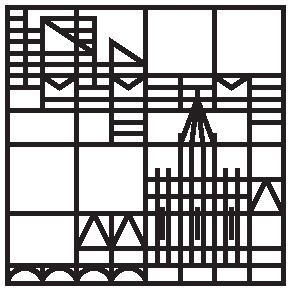
\includegraphics[width=5cm]{logo}
\\ \Large Universität Konstanz  \\ \vspace{4ex} \huge 
Skript zur Vorlesung\\ Höhere Quantentheorie und Elektrodynamik
\\ \vspace{4ex} \Large Prof. Dr. Wolfgang Belzig 
\\ Version vom 30. Juli 2012 \\ \vspace{4.5cm}
\normalsize Ursprünglichen Mitschrift von Birte Heinze im WS 09/10 \\ Ausführliche Überarbeitung von Tobias Lohse im WS 11/12 \vspace{-10cm}}
\author{}
\date{}
%\begin{document}

\subsection{Zeitabhängige Störungstheorie}
Näherungsmethoden stellen in der theoretischen Physik ein äußerst wichtiges Instrument dar, da nur die allerwenigsten und einfachsten Systeme direkt analytisch lösbar sind. Die Störungstheorie ist dabei das am häufigsten anwendbare Verfahren und beruht auf dem Grundgedanke den Hamiltonoperator eines Systems $\hat{\ham}$ durch den Hamiltonoperator $\hat{\ham}_0$ eines Systems anzunähern, dessen Lösung bereits bekannt ist und den Restterm, die {\bf Störung} $\hat{\ham}-\hat{\ham}_0=\lambda\hat{\ham}'$, in einer Potenzreihe zu entwickeln um deren Einfluss auf die Lösung anzunähern. Dieses Verfahren funktioniert immer dann gut, wenn der Einfluss der Störung $\lambda\hat{\ham}'$ auf das Gesamtsystem $\hat{\ham}=\hat{\ham}_0+\lambda\hat{\ham}'$ gering ist. In diesem Abschnitt soll insbesondere auf die Störungstheorie für einen zeitabhängigen Störterm $\hat{\ham}'(t)$ eingegangen werden. Dies ist beispielsweise relevant, wenn der Einfluss von Rauschen auf ein System untersucht werden soll. 

\subsubsection{Zeitabhängigkeit in der Schrödingertheorie}
Zunächst soll an dieser Stelle auf die Zeitabhängigkeit in der Schrödingertheorie eingegangen werden. Diese ergibt sich aus der Lösung der zeitabhängigen Schrödingergleichung (\ref{SG}): $\I\hbar\;\partial_t\ket{\psi(t)}=\hat{\ham}(\hat{\vec{p}},\hat{\vec{r}},t)\ket{\psi(t)}$. Im Normalfall hat der Hamiltonoperator dabei folgende Form: $\hat{\ham}(\hat{\vec{p}},\hat{\vec{r}},t) = T(\hat{\vec{p}}) + \hat{V}(\hat{\vec{r}},t)$. Im Falle eines zeitunabhängigen Potentials $\hat{V}(\hat{\vec{r}},t)=\hat{V}(\hat{\vec{r}})$ lässt sich die Zeitabhängigkeit wie bereits im ersten Abschnitt erwähnt in einen Phasenfaktor abseparieren $\ket{\psi(t)}=\exp(\I E t/\hbar)\ket{\psi}$. Die Schrödingergleichung wird dann zu einem zeitunabhängigen Eigenwertproblem (\ref{statSG}): $\hat{\ham}\ket{\psi}=E\ket{\psi}$. Deren Lösungen die Eigenzustände $\ket{\psi_n}$ mit den zugehörigen Eigenenergien $E_n$ sind. Die Allgemeine Lösung ergibt sich aus dem Superpositionsprinzip zu: 
\begin{eqnarray*}
	\ket{\psi(t)} = \sum_n c_n\cdot \e^{\frac{\I}{\hbar}E_n t}\ket{\psi_n}
\end{eqnarray*}
Die $c_n$ sind dabei komplexe Koeffizienten, die allein von den Anfangsbedingungen abhängen. 

Besitzt das Potential einen zeitabhängigen Teil $\hat{V}(\hat{\vec{r}},t)=\hat{V}_0(\hat{\vec{r}})+\hat{V}(\hat{\vec{r}},t)$, so kann der Hamiltonoperator in einen zeitunabhängigen und einen zeitabhängigen Teil aufgeteilt werden: $\hat{\ham}(\hat{\vec{p}},\hat{\vec{r}},t)=\hat{\ham}_0(\hat{\vec{p}},\hat{\vec{r}})+\hat{V}(\hat{\vec{r}},t)$. Da die Eigenzustände $\ket{\psi_n^{(0)}}$ des stationären Teils $\hat{\ham}_0$ eine vollständige Basis des Hilbertraums des Systems bilden, kann als Lösungsansatz folgendes verwendet werden: 
\begin{eqnarray*}
	\ket{\psi(t)} = \sum_n c_n(t)\cdot\ket{\psi_n^{(0)}}
\end{eqnarray*}
Die zeitabhängigen Koeffizienten $c_n(t)$ können nun durch einsetzten in die Schrödingergleichung gefunden werden. Dazu müssen $N$ Differenzialgleichungen erster Ordnung gelöst werden, deren Anfangsbedingungen bekannt sein sollten. $N$ ist dabei die Anzahl der Eigenzustände von $\hat{\ham}_0$.


\subsubsection{Zeitunabhängige Störungstheorie}
Wir wollen zunächst kurz auffrischen, wie im Falle einer zeitunabhängigen Störung die Störungstheorie funktioniert. Wir gehen also davon aus, dass sich der Hamiltonoperator $\hat{\ham}$ aufteilen lässt in einen Teil $\hat{\ham}_0$, dessen Lösung bekannt ist, und eine Störung $\lambda\hat{V}$. Der Parameter $\lambda$ hat hierbei keine besondere Bedeutung, es handelt sich lediglich um einen dimensionsloser Entwicklungsparameter. Wir schreiben den Hamiltonoperator also wie folgt: 
\begin{eqnarray*}
	\hat{\ham} = \hat{\ham}_0+\lambda \hat{V}
\end{eqnarray*}
Wir wollen nun die Eigenzustände $\ket{\psi_n}$ und Eigenenergien $E_n$ des gesamten Systems in einer Potenzreihe im Parameter $\lambda$  entwickeln: 
\begin{eqnarray*}
	E_n &=& E_n^{(0)} + \lambda E_n^{(1)} + \lambda^2 E_n^{(2)} + \ldots \;=\;  \sum_{k=0} \;\lambda^k E_n^{(k)}
	\\
	\ket{\psi_n} &=& \ket{\psi_n^{(0)}} + \lambda\ket{\psi_n^{(1)}} + \lambda^2 \ket{\psi_n^{(2)}} + \ldots \;=\; \sum_{k=0} \;\lambda^k \ket{\psi_n^{(k)}}
\end{eqnarray*}
Dabei sind die $\ket{\psi_n^{(0)}}$ und zugehörigen $E_n^{(0)}$ die bekannten Eigenzustände und Eigenenergien des ungestörten Hamiltonoperators. Die Eigenzustände des hermiteschen Operators $\hat{\ham}_0$ stellen eine vollständiges Orthonormalsystem $\braket{\psi_n^{(0)}}{\psi_m^{(0)}}=\delta_{n,m}$ dar und wir können die Normierung zweckmäßig auf $\braket{\psi_n^{(0)}}{\psi_n}=1$ festlegen. Falls die Eigenwerte nicht entartet sind, folgt unmittelbar, dass $\braket{\psi_n^{(0)}}{\psi_n^{(k)}}=\delta_{0,k}$ gilt. Wenn wir nun den Ansatz in die stationäre Schrödingergleichung (\ref{statSG}) einsetzen und nach Potenzen in $\lambda$ ordnen, so lassen sich durch Multiplikation der Gleichung mit $\bra{\psi_n^{(0)}}$ die Energien in den verschiedenen Ordnungen bestimmen als: 
\begin{eqnarray*}
	E_n^{(k)} &=& \bracket{\psi_n^{(0)}}{\lambda\hat{V}}{\psi_n^{(k-1)}}
\end{eqnarray*}
Um die Zustände $\ket{\psi_n^{(k)}}$ höherer Ordnung zu erhalten, multiplizieren wir die Gleichung mit $\bra{\psi_m^{(0)}}$ mit $m\neq n$. Für die Zustandskorrektur in erster Ordnung ergibt sich dann: 
\begin{eqnarray*}
	\ket{\psi_n^{(1)}} &=& \sum_{m\neq n} \; \frac{|\bracket{\psi_m^{(0)}}{\lambda\hat{V}}{\psi_n^{(0)}}|}{E_n^{(0)}-E_m^{(0)}}\cdot \ket{\psi_n^{(0)}}
\end{eqnarray*}
Im Falle einer Entartung des Eigensystems von $\hat{\ham}_0$ muss $\lambda\hat{V}$ zunächst im Unterraum der entarteten Zustände diagonalisiert werden, bevor die Störungstheorie angewandt werden kann. 


\subsubsection{Darstellung der Zeitabhängigkeiten in der Quantenmechanik}
Zeitabhängigkeiten können auf Grund der speziellen Struktur des Formalismus der Quantenmechanik auf verschiedene Art und Weise ausgedrückt werden. Man unterscheidet hauptsächlich drei Konventionen zur Zeitabhängigkeit von Zuständen und Observablen in der Quantenmechanik: 
\begin{itemize1}
	\item Das {\bf Schrödinger-Bild}, in dem wir bisher gearbeitet haben und in welchem die Zustände Zeitabhängig sind.  
	\item Das {\bf Heisenberg-Bild}, indem die Zeitabhängigkeit in die Observablen verschoben wird. 
	\item Das {\bf Dirac-Bild} oder {\bf Wechselwirkungsbild}, in welchem die Zeitentwicklung sowohl in den Observablen als auch in den Zuständen vorkommt. 
\end{itemize1}
Alle drei Konventionen können für die Lösung bestimmter Probleme vorteilhaft sein. Im allgemeinen sind die verschiedenen Bilder allerdings völlig gleichberechtigt. 

Im folgenden sollen die drei Bilder und ihre Unterschiede etwas genauer erläutert werden: 

\paragraph{Das Schrödinger-Bild}

Bisher haben wir uns ausschließlich mit dem Schrödinger-Bild befasst. In folgenden sollen dessen wichtigste Eigenschaften noch einmal zusammen gefasst werden:

\begin{itemize1}
	\item Die Zustandsvektoren sind zeitabhängig $\ket{\psi(t)}$. Die Zeitentwicklung der Zustandsvektoren wird durch die Schrödingergleichung beschrieben: $\I\hbar\;\dell_t\ket{\psi(t)} = \hat{\ham}(t) \ket{\psi(t)}$
	\item Operatoren $\hat{A}(t)$ können explizit von der Zeit abhängen, sind aber keiner Zeitentwicklung unterworfen. 
	\item Der Erwartungswert eines Operators ist das gemittelte Messergebnisse der Observablen und berechnet sich damit als $\EW{\hat{A}(t)} = \bracket{\psi(t)}{\hat{A}(t)}{\psi(t)}$. 
	\item Für zeitunabhängigen Hamiltonoperatoren $\hat{\ham(t)}=\hat{\ham}_0$ ist eine formale Lösung der Schrödingergleichung gegeben durch: 
	\begin{eqnarray*}
		\ket{\psi(t)} &=& \underbrace{\e^{-\frac{\I}{\hbar}\cdot\hat{\ham}_0\;t}}_{=\hat{U}_0} \ket{\psi(0)} = \hat{U}_0\ket{\psi(0)}
	\end{eqnarray*}
	Der Operator $\hat{U}_0=\exp(-\I/\hbar\cdot\hat{\ham}_0\;t)$ wird dabei als unitärer {\bf Zeitentwicklungsoperator} des zeitunabhängigen Hamiltonoperators $\hat{\ham}_0$ bezeichnet. Unitäre Operatoren erfüllen die Gleichung $\hat{U}^{\dagger}\hat{U}=\hat{U}\hat{U}^{\dagger}=1$. 
\end{itemize1}

\paragraph{Das Heisenberg-Bild}

Im Heisenberg-Bild wird die Zeitabhängigkeit in die Operatoren verschoben. Operatoren und Zustände im Heisenberg-Bild werden häufig mit einem Index $_H$ versehen um sie als solche zu kennzeichnen. Der Formalismus ist durch folgende Definitionen und Eigenschaften gekennzeichnet: 

\begin{itemize1}
	\item Der Zustandsvektor im Heisenberg-Bild ist definiert als: 
	\begin{eqnarray*}
		\ket{\psi_H} &=& \hat{U}^{\dagger}\ket{\psi(t)} \quad=\quad \ket{\psi(0)}
	\end{eqnarray*}
	Damit sind die Zustandsvektoren zeitunabhängig und die Zeitentwicklung kann nicht mehr durch die Schrödingergleichung beschrieben werden. 
	\item Der unitäre Zeitentwicklungsoperator $\hat{U}$ ist dabei im einfachsten Fall eines zeitunabhängigen Hamilton Operators $\hat{\ham}_0$ gegeben durch $\hat{U}_0(t)=\exp(-\I/\hbar\cdot\hat{\ham}_0\;t)$, im Falle eines zeitabhängigen Hamilton Operators kann er ebenfalls definiert werden, seine Darstellung wird allerdings komplizierter. Die definierende Bestimmung für den Zeitentwicklungsoperator ist die Differentialgleichung $\I\hbar \dell_t \hat{U}(t)=\hat{\ham}(t)\hat{U}(t)$. Mehr zu deren allgemeiner Lösung im übernächsten Paragraph. 
	\item Die Operatoren im Heisenberg-Bild sind definiert als: 
	\begin{eqnarray*}
		\hat{A}_H(t) &=& \hat{U}^{\dagger}\;\hat{A}(t)\;\hat{U}
	\end{eqnarray*}
	\item Der Erwartungswert muss in allen Bildern gleich bleiben. Dies lässt sich leicht zeigen: $\EW{\hat{A}}=\bracket{\psi(t)}{\hat{A(t)}}{\psi(t)}=\bracket{\psi(0)}{\hat{U}^{\dagger}\hat{A}(t)\hat{U}}{\psi(0)}=\bracket{\psi_H}{\hat{A}_H(t)}{\psi_H}$. 
	\item Die Zeitentwicklung ist im Heisenberg-Bild durch eine Operator-Gleichung bestimmt, welche sich aus der Definition des Zeitentwicklungsoperators ergibt als: 
	\begin{eqnarray}
		\frac{\mathrm{d}}{\mathrm{d}t} \hat{A}_H(t) &=& \frac{\mathrm{d}}{\mathrm{d}t} \Big(\hat{U}^{\dagger}(t)\hat{A}(t)\hat{U}(t)\Big) = \hat{U}^{\dagger}\Big(\underbrace{\frac{\I}{\hbar}\hat{\ham}\hat{A}(t)-\frac{\I}{\hbar}\hat{A}(t)\hat{\ham}}_{=\I/\hbar\cdot[\hat{\ham},\hat{A}(t)]}+\dell_tA(t)\Big)\hat{U} \nonumber
		\\
		&=& \frac{\I}{\hbar}\cdot[\hat{H},\hat{A}_H(t)]+\big(\dell_tA(t)\big)_H \label{HG}
	\end{eqnarray}
	Diese Gleichung wird auch als {\bf Heisenberg Gleichung} bezeichnet. Man beachte außerdem, dass selbstverständlich $[\hat{H},\hat{A}_H(t)]=\big([\hat{H},\hat{A}(t)]\big)_H$ gilt, da der Hamiltonoperator mit dem Zeitentwicklungsoperator vertauscht. 
\end{itemize1} 


\paragraph{Das Wechselwirkungsbild}

Für Probleme mit zeitabhängigem Hamiltonoperator $\hat{\ham}(t)=\hat{\ham}_0+\hat{V}(t)$ eignet sich die Einführung eines gemischten Bildes, in dem sowohl Zustände als auch Operatoren teilweise zeitabhängig sind. Dieses Bild wird als Wechselwirkungsbild oder Dirac-Bild bezeichnet und die Zustände und Operatoren werden häufig mit einem Index $_I$ für englisch 'interaction' gekennzeichnet. Folgendes sind die essentiellen Definitionen: 

\begin{itemize1}
	\item Das Wechselwirkungsbild ist in einem System mit einem zeitabhängigen Hamiltonoperator $\hat{\ham}(t)$ definiert, welcher aus einem zeitunabhängigen Teil $\hat{\ham}_0$ und einem zeitabhängigen Teil $\hat{V}(t)$ zusammengesetzt ist: 
	\begin{eqnarray*}
		\hat{\ham}(t) &=& \hat{\ham}_0+\hat{V}(t) 
	\end{eqnarray*}
	Für den zeitunabhängigen Teil des Hamiltonoperators wird der Zeitentwicklungsoperator $\hat{U}_0=\exp(-\I/\hbar\cdot \hat{\ham}_0t)$ definiert. 
	\item Die Zustände im Wechselwirkungsbild sind wie folgt definiert: 
	\begin{eqnarray*}
		\ket{\psi_I(t)} &=& \hat{U}_0^{\dagger}\ket{\psi(t)} \;=\; \e^{\;\frac{\I}{\hbar}\; \hat{\ham}_0\; t}\ket{\psi(t)}
	\end{eqnarray*}
	\item Die Operatoren im Wechselwirkungsbild sind definiert als: 
	\begin{eqnarray*}
		\hat{A}_I(t) &=& \hat{U}^{\dagger}_0\;\hat{A}(t)\;\hat{U}_0
	\end{eqnarray*}
	\item Die Bewegungsgleichung im Wechselwirkungsbild ergibt sich aus der Schrödingergleichung: 
	\begin{eqnarray}
		\I\hbar\;\dell_t \ket{\psi_I(t)} &=& \I\hbar\;\dell_t \;\Big(\hat{U}^{\dagger}_0(t) \ket{\psi(t)}\Big) = \hat{U}^{\dagger}_0 \big(\I\hbar\;\dell_t-\hat{\ham}_0\big)\ket{\psi(t)} = \hat{U}^{\dagger}_0\big(\underbrace{\hat{\ham}-\hat{\ham}_0}_{=\hat{V}(t)}\big)\underbrace{\hat{U}_0 \hat{U}^{\dagger}_0}_{=\1} \ket{\psi(t)} \nonumber
		\\
		&=& \hat{V}_I(t) \ket{\psi_I(t)} \label{WechselwirkungsbildSG}
	\end{eqnarray}
	Die Zeitentwicklung in Wechselwirkungsbild ist also allein durch $\hat{V}_I$ bestimmt. 
\end{itemize1}

\subsubsection{Allgemeine Lösung der Schrödingergleichung im Wechselwirkungs}

Wir wollen nun die Schrödingerlgeichung des Wechselwirkungsbilds (\ref{WechselwirkungsbildSG}) ganz allgemein lösen. Dazu verwenden wir die Anfangsbedingungen $\ket{\psi_I(0)}=\ket{\psi(0)}=:\ket{\psi_0}$ und integrieren Schrödingerlgeichung des Wechselwirkungsbilds (\ref{WechselwirkungsbildSG}): 
\begin{eqnarray*}
	\ket{\psi_I(t)} &=& \ket{\psi_0} - \frac{\I}{\hbar}\int_0^t \mathrm{d}t'\; \hat{V}_I(t') \ket{\psi_I(t')} 
\end{eqnarray*}
Wenn wir nun die linke Seite in die Rechte einsetzen erhalten wir folgende Gleichung: 
\begin{eqnarray*}
	\ket{\psi_I(t)} &=& \ket{\psi_0} - \frac{\I}{\hbar}\int_0^t\mathrm{d}t'\; \hat{V}_I(t') \ket{\psi_0} + \Big(\frac{-\I}{\hbar}\Big)^2 \int_0^t \mathrm{d}t'\; \int_0^{t'}\mathrm{d}t''\; \hat{V}_I(t')\hat{V}_I(t'')\ket{\psi_I(t'')}
\end{eqnarray*}
Durch wiederholtes Einsetzten der linken Seite in die rechte, entsteht eine unendliche Summe und die Gleichung erhält folgende Form:
\begin{eqnarray*}
	\ket{\psi_I(t)} &=& \underbrace{\sum_{n=0}^{\infty} \Big(\frac{-\I}{\hbar}\Big)^n \int_0^t\mathrm{d}t_1 \int_0^{t_1}\mathrm{d}t_2\;\; \cdots \int_0^{t_{n-1}}\mathrm{d}t_n\; \hat{V}_I(t_1)\hat{V}_I(t_2) \cdots \hat{V}_I(t_n)}_{=:\;\hat{U}_I(t,0)} \ket{\psi_0}
\end{eqnarray*}
Damit haben wir einen Zeitentwicklungsoperator $\hat{U}_I(t,0)$ für das Potential $\hat{V}_I(t)$ definiert. Dabei ist auf die Zeitordnung zu achten, da die Operatoren $\hat{V}_I(t_i)$ zu verschiedenen Zeiten $t_i$ nicht notwendigerweise vertauschen. Der Operator mit dem kleinsten Zeitparameter steht am weitesten rechts: $t\geq t_1\geq t_2\geq \cdots \geq t_n\geq 0$. Um diesem Umstand Rechnung zu tragen führen wir daher den Dysonschen {\bf Zeitordnungsoperator} $\widehat{T}$ ein, welcher zwei Operatoren vertauscht, auch wenn deren Kommutator nicht null ist:
\begin{eqnarray*}
	\widehat{T}\big(\hat{A}(t)\hat{B}(t')\big) = \left\{ \begin{array}{rl} \hat{A}(t)\hat{B}(t') & t > t'\\\hat{B}(t')\hat{A}(t) & t < t'\end{array}\right. 
\end{eqnarray*}
Mit Hilfe des Zeitordnungsoperators lässt sich nun die Gleichung wie folgt umformen:
\begin{eqnarray*}
	&&\!\!\!\!\! \widehat{T}\;\bigg( \int_0^{t}\mathrm{d}t_1 \int_0^{t_1}\mathrm{d}t_2\;\cdots\int_0^{t_{n-1}}\mathrm{d}t_n\; \hat{V}_I(t_1)\hat{V}_I(t_2) \cdots \hat{V}_I(t_n) \bigg)
	\\
	&&\!=\;\widehat{T}\;\bigg( \frac{1}{n!}\cdot \int_0^{t}\mathrm{d}t_1 \int_0^{t}\mathrm{d}t_2\;\cdots\int_0^{t}\mathrm{d}t_n\; \hat{V}_I(t_1)\hat{V}_I(t_2) \cdots \hat{V}_I(t_n) \bigg) \;=\; \widehat{T}\;\Bigg( \frac{1}{n!}\cdot \bigg(\int_0^{t}\mathrm{d}t'\; \hat{V}_I(t')\bigg)^n \Bigg)
\end{eqnarray*}
Die Korrektheit des Faktors $1/n!$, welcher bei der Erweiterung der Integrale auftaucht, lässt sich beweisen, indem die Gleichung nach $t$ abgeleitet wird. Der Zeitentwicklungsoperator $\hat{U}_I(t,0)$ lässt sich damit nun sehr kompakt schreiben als: 
\begin{eqnarray}
	\hat{U}_I(t,0) &=& \widehat{T}\;\Bigg( \sum_{n=0}^{\infty} \cdot \frac{1}{n!}\cdot \bigg(\!\!-\frac{\I}{\hbar}\cdot\int_0^{t}\mathrm{d}t'\; \hat{V}_I(t')\bigg)^n \Bigg) \;=\;\; \widehat{T}\;\exp \bigg(\!\!-\frac{\I}{\hbar}\cdot\int_0^{t}\mathrm{d}t'\; \hat{V}_I(t')\bigg) \qquad\label{Zeitentwicklungsoperator}
\end{eqnarray}
Somit haben wir eine allgemeine Form des Zeitentwicklungsoperators hergeleitet. Im folgenden sollen dessen Eigenschaften zusammen gefasst werden: 

\begin{itemize1}
	\item Der Zeitentwicklungsoperator stellt die Lösung der folgenden Differentialgleichung dar, welche sich direkt aus der Schrödingergleichung ableitet:
	\begin{eqnarray*}
		\I\hbar\;\dell_t\;\hat{U}_I(t,0) = \hat{U}_I(t,0)\;\hat{V}_I(t)
	\end{eqnarray*}
	Da bei der Lösung dieser Differentialgleichung keine Annahmen über die Form von $\hat{V}_I$ getroffen wurden, stellt die Definition in Gleichung (\ref{Zeitentwicklungsoperator}) die allgemeine Definition eines Zeitentwicklungsoperators $\hat{U}$ eines Quantenmechanischen Systems mit einem beliebigen Hamiltonoperator $\hat{\ham}(t)=\hat{V}_I(t)$ dar, welcher beispielsweise für die Formulierung des Heisenberg-Bilds genutzt werden kann. 
	\item Für zeitunabhängige Hamiltonoperatoren $\hat{V}_I(t)=\hat{\ham}$ ergibt sich sofort der bereits bekannte Zeitentwicklungsoperator: $\hat{U}_0=\widehat{T}\exp(-\I/\hbar\cdot\int_0^t\mathrm{d}t'\;\hat{\ham}_0) = \exp(-\I/\hbar\cdot \hat{\ham}_0\;t)$. 
	\item Es gilt wie man leicht sieht $\hat{U}_I(t,t) = \1$. 
	\item Der Zeitentwicklungsoperator zwischen zwei Zeitpunkten $t$ und $t'$ kann wie man leicht sieht immer auf folgende weise zusammengesetzt werden: $\hat{U}_I(t,t')=\hat{U}_I(t,t'') \hat{U}_I(t'',t')$:
	\item Falls für alle $t,t'$ gilt $[\hat{V}_I(t),\hat{V}_I(t')]=0$, so wird der Zeitordnungsoperator $\widehat{T}$ in Gleichung (\ref{Zeitentwicklungsoperator}) überflüssig.
	\item Da der Zeitentwicklungsoperator durch eine Potenzreihe gegeben ist, kann sich die Zeitentwicklung nähern lassen, wenn wir die Potenzreihe ab einer bestimmten Ordnung abbrechen lassen. 
	\item In der niedrigsten Ordnung ist der Zeitordnungsoperator $\widehat{T}$ ebenfalls überflüssig und der Zeitenetwicklungsoperator ergibt sich zu: $\hat{U}_I(t,0) = \1-\I/\hbar\cdot\int_0^t\mathrm{d}t'\; \hat{V}_I(t')$
	\item Es lässt sich außerdem zeigen, dass folgendes gilt: $\hat{U}_I(t,0)-\1 = \hat{U}_I^{\dagger}(t,0) = \hat{U}_I(0,t)$. 
\end{itemize1}


\subsubsection{Übergangswahrscheinlichkeiten}

Anstatt die gesamte Zeitentwicklung eines Systems zu berechnen ist es häufig interessant einfach nur die Übergangswahrscheinlichkeit von einem Zustand in einen anderen zu berechnen, wenn das System gestört wird. 

Dies wollen wir im folgenden Abschnitt für ein System mit zeitunabhängigem Hamiltonoperaotr $\hat{\ham}_0$ und eine zeitabhängige Störung $\hat{V}(t)$ tun, welche zum Zeitpunkt $t=0$ eingeschaltet wird: $\hat{V}(t<0)=0$. Eine solch Störung könnte beispielsweise ein für eine gewisse Zeitspanne eingeschaltetes äußeres Feld oder der Vorbeiflug eines geladenen Teilchens sein. Das System befindet sich also zum Zeitpunkt $t=0$ in einem Initialzustand $\ket{i}$. Die Übergangswahrscheinlichkeit $P_{i\to f}(t)$ in einem Finalzustand $\ket{f}$ zum Zeitpunkt $t$ ist dann gegeben durch: 
\begin{eqnarray*}
	P_{i\to f}(t) &=& \big|\braket{f}{\psi(t)}\big|^2 = \big|\bracket{f}{\hat{U}_0}{\psi_I(t)} = \big|\bracket{f}{\e^{-\frac{\I}{\hbar}\cdot \hat{\ham}_0\;t}}{\psi_I(t)}\big|^2
\end{eqnarray*}
Wobei $\ket{\psi(t)}$ der Zustand des Systems zum Zeitpunkt $t$ ist. Wenn der Finalzustand $\ket{f}$ nun ein Eigenzustand des zeitunabhängigen Hamiltonoperators mit Eigenenergie $E_f$ ist, so verursacht $\hat{U}_0$ nur eine Phasenverschiebung, welche den Betrag nicht ändert: 
\begin{eqnarray*}
	P_{i\rightarrow f}(t)=\big|\bracket{f}{\e^{-\frac{\I}{\hbar}\cdot \hat{\ham}_0\;t}}{\psi_I(t)}\big|^2 = \big|\e^{-\frac{\I}{\hbar}\cdot E_f\;t}\cdot\braket{f}{\psi_I(t)}\big|^2 &=& \big|\braket{f}{\psi_I(t)}\big|^2 = \big|\bracket{f}{\hat{U}_I}{i}\big|^2 
\end{eqnarray*}
Für den Fall, dass $\ket{i}$ und $\ket{f}$ orthogonal zueinander sind: $\braket{i}{f}=0$ und auch $\ket{i}$ ein Eigenzustand von $\hat{\ham}_0$ mit Eigenenergie $E_i$ ist ergibt sich dann in Näherung erster Ordnung für $\hat{U}_I$, also für relativ kleine Störpotentiale und relativ kleine Zeitintervalle $t$ die Übergangswahrscheinlichkeit zu: 
\begin{eqnarray}
	P_{i\to f}(t) &\approx& \Big|\braket{f}{i} - \frac{\I}{\hbar} \int_0^t\mathrm{d}t'\; \bracket{f}{\hat{V}_I(t')}{i} \Big|^2 = \frac{1}{\hbar^2}\cdot \Big|\int_0^t\mathrm{d}t'\; \bracket{f}{\hat{U}^{\dagger}_0(t')\;\hat{V}(t')\;\hat{U}_0(t')}{i} \Big|^2 \nonumber
	\\
	&& \qquad\qquad= \frac{1}{\hbar^2}\cdot \Big|\int_0^t\mathrm{d}t'\; \exp\Big(\I\cdot\underbrace{\frac{E_f-E_i}{\hbar}}_{=:\;\omega_{fi}}\cdot t'\Big) \cdot\bracket{f}{\hat{V}(t')}{i} \Big|^2 \nonumber
	\\
	\Rightarrow\quad P_{i\to f}(t) &\approx& \frac{1}{\hbar^2}\cdot \Big|\int_0^t\mathrm{d}t'\; \e^{\;\I\;\omega_{fi}\cdot t'} \cdot\bracket{f}{\hat{V}(t')}{i}\;\Big|^2 \label{Uebergangswahrscheinlichkeit} 
\end{eqnarray} 
Wir haben somit eine recht einfache Näherung für die Übergangswahrscheinlichkeit zwischen zwei orthogonalen Eigenzuständen $\ket{i}$ und $\ket{f}$ des zeitunabhängigen Hamiltonoperators unter Einfluss einer zeitlichen Störung $\hat{V}(t)$ gefunden. Die Näherung funktioniert nicht, falls $P_{i\rightarrow f}(t)\approx0$ gilt. 


\paragraph{Konstante Störung}

Übergangswahrscheinlichkeit im Falle eines nach dem Einschalten zeitlich konstanten Potentials untersuchen. Mit Hilfe der Theta-Funktion $\Theta(t>0)=1\land\Theta(t<0)=0$, lässt sich dieses schreiben als: $\hat{V}(t)=\Theta(t)\cdot\hat{V}$. Gleichung (\ref{Uebergangswahrscheinlichkeit}) lässt sich in diesem Fall vereinfachen zu:  
\begin{eqnarray*}
	P_{i\to f}(t,\omega_{fi}) = \underbrace{\frac{1}{\hbar^2}\cdot\big|\bracket{f}{\hat{V}}{i}\big|^2 }_{=:\;M_{fi}} \cdot 
	\Big|\int_0^t\mathrm{d}t'\; \e^{\;\I\;\omega_{fi}\cdot t'} \Big|^2 = M_{fi} \cdot \Big| \frac{\e^{\;\I\;\omega_{fi}\cdot t'}-1}{\I\;\omega_{fi}}\Big|^2 =\; M_{fi} \cdot\frac{\sin^2\big(\frac{\omega_{fi}}{2}\cdot t\big)}{\big(\frac{\omega_{fi}}{2}\big)^2}
\end{eqnarray*}
Die Übergangswahrscheinlichkeit hängt also linear vom Matrixelement $M_{fi}$ ab und wird maximal für kleine $\omega_{fi}$, also für Zustände mit nur wenig unterschiedlichen Energieeigenwerten. Die Übergangswahrscheinlichkeit wird null für $\omega_{fi}=2\pi/t\cdot n$ mit $n\in\mathbb{N}$ und wird für große $\omega_{fi}$ sehr schnell klein, die Halbwertsbreite ist proportional zu $1/t$. Das Maximum von $P_{i\to f}(t,\omega_{fi})$ ergibt sich für $\omega_{fi}\to0$ mit l'Hospitale zu: 
\begin{eqnarray*}
	\max\big(P_{i\to f}(t)\big) &=& \lim_{\omega_{fi}\to0}M_{fi}\cdot\frac{\sin^2\big(\frac{\omega_{fi}}{2}\cdot t\big)}{\big(\frac{\omega_{fi}}{2}\big)^2}= M_{fi}\cdot t^2 = \frac{1}{\hbar^2}\cdot\big|\bracket{f}{\hat{V}}{i}\big|^2 \cdot t^2
\end{eqnarray*}
Der folgende Plot soll das Verhalten von $P_{i\to f}(t,\omega_{fi})$ noch einmal veranschaulichend darstellen:
\vspace{-2ex}\begin{figure}[!h]\center
	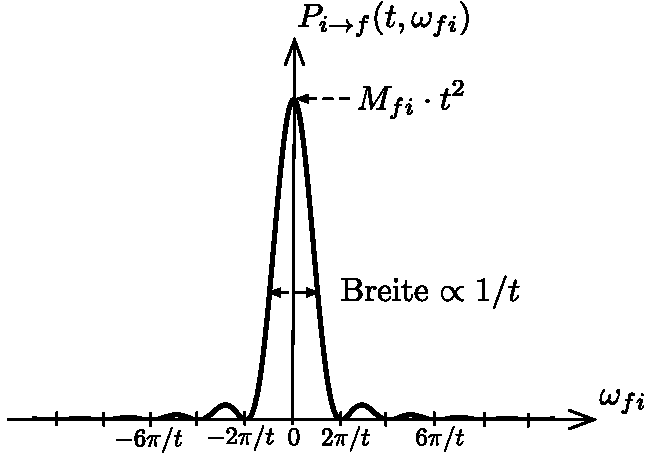
\includegraphics[scale=.75]{Figs/Sin2Plot}
\end{figure}\vspace{-4ex}

Interessant ist der Grenzfall für lange Zeiten $t\to\infty$. Für diesen können wir, wenn wir $\omega_{fi}:=\alpha$ substituieren, die folgende Funktionenfolge $\delta_t(\alpha)$ definieren: 
\begin{eqnarray*}
	P_{i\to f}(t,\omega_{fi}) = M_{fi}\cdot\pi\cdot t\cdot \frac{\sin^2\big(\frac{\omega_{fi}}{2}\cdot t\big)}{\pi \big(\frac{\omega_{fi}}{2}\big)^2\cdot t} = M_{fi}\cdot\pi\cdot t\cdot\underbrace{\frac{\sin^2(\alpha\cdot t)}{\pi\alpha^2\cdot t}}_{=:\;\delta_t(\alpha)} = M_{fi}\cdot\pi\cdot t\cdot \delta_t(\alpha)
\end{eqnarray*}
Die Funktionenfolge $\delta_t(\alpha)$ hat in einem Kontinuum folgende Eigenschaft: 
\begin{eqnarray*}
	\lim_{t\to\infty}\int_{-\infty}^{\infty}\mathrm{d}\alpha\;\delta_t(\alpha)\cdot F(\alpha) = \lim_{t\to\infty}\frac{1}{\pi}\underbrace{\int_{-\infty}^{\infty}\mathrm{d}y\;\frac{\sin^2y}{y^2}}_{=\;\pi}\cdot F(y/t) = F(0)
\end{eqnarray*}
Für $t\to\infty$ ist $\delta_t(\alpha)$ also eine Darstellung der Deltafunktion. Damit ergibt sich dann die Übergangswahrscheinlichkeit, wenn $\omega_{fi}$ als Kontinuum betrachtet werden kann zu: 
\begin{eqnarray*}
	\lim_{t\to\infty}P_{i\to f}(t) &=& M_{fi}\cdot\pi\cdot t\cdot \delta\Big(\frac{E_f-E_i}{2\hbar}\Big) = 2\pi\hbar\cdot M_{fi}\cdot t\cdot \delta(E_f-E_i)
\end{eqnarray*}
Für eine lange andauernde relativ kleine Störung in einem kontinuierlichen Energiespektrum haben wir somit eine einfache Darstellung für die {\bf Übergangsrate} $\Gamma_{i\to f}=\dell_t\;P_{i\to f}$ gefunden, welche in zahlreichen physikalischen Problemen sehr nützlich ist und auch als {\bf Fermis Goldene Regel} bezeichnet wird: 
\begin{eqnarray}
	\Gamma_{i\to f} =  \frac{2\pi}{\hbar}\cdot\big|\bracket{f}{\hat{V}}{i}\big|^2 \cdot \delta(E_f-E_i) \label{FermisGoldeneRegel}
\end{eqnarray}
Dabei mag es vielleicht zunächst etwas verwirrend erscheinen, dass wir für die Herleitung von (\ref{Uebergangswahrscheinlichkeit}) in erster Ordnung der zeitabhängigen Störungstheorie angenommen haben, dass das Zeitintervall $t$ relativ klein ist und nun eine Näherung für $t\to\infty$ gemacht haben, was in einer mit der Zeit unbegrenzt linear anwachsenden Überganswahrscheinlichkeit resultiert ist. Dies ist natürlich nur zulässig sofern die Störung innerhalb des Zeitintervalls $t$ klein bleibt: $|\bracket{i}{\hat{V}}{f}|^2\cdot t\ll1$. Die Näherung durch die Deltafunktion wird legitim, wenn die Breite der Funktion $P_{i\to f}(E_f-E_i)$, welche wir auf halbem Weg zum ersten Minimum als $2\pi\hbar/t$ abschätzen können (Man beachte $E_f-E_i=2\cdot\hbar\omega_{fi}$), deutlich kleiner ist als die Breite der kontinuierlichen Energieverteilung $\Delta\varepsilon$. Andererseits muss die Anzahl der Zustände innerhalb des Peaks von $P_{i\to f}(E_f-E_i)$ groß genug sein, um die Energie als Kontinuum zu nähern, das heißt der Abstand zwischen den einzelnen Energien $\delta\varepsilon$ muss viel kleiner als $2\pi\hbar/t$ sein. Im folgenden Plot ist die Funktion $P_{i\to f}(E_f-E_i)$ in der Energieverteilung mit Breite $\Delta\varepsilon$ mit den einzelnen Energien im Abstand $\delta\varepsilon$ noch einmal schematisch dargestellt: 
\vspace{-2ex}\begin{figure}[!h]\center
	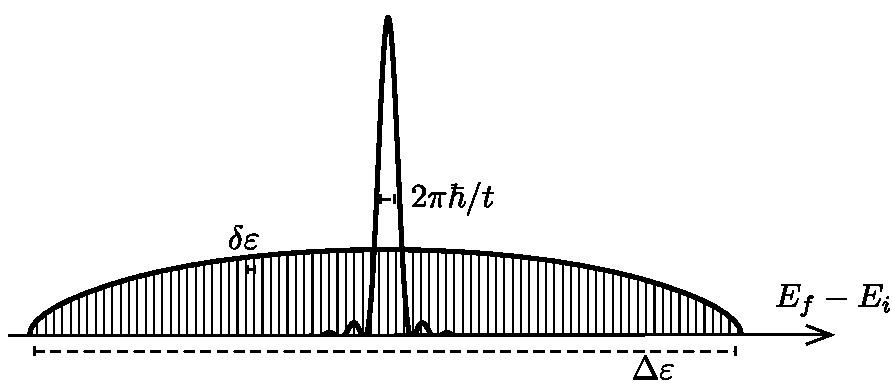
\includegraphics[scale=.75]{Figs/Escale}
\end{figure}\vspace{-4ex} 

Die Bedingung für den Zeitmaßstab in der Kontinuums und Deltapeak Näherung lautet also zusammengefasst wie folgt: 
\begin{eqnarray*}
	\frac{2 \pi \hbar}{\delta\varepsilon} \quad\gg\quad t \quad\gg\quad \frac{2\pi \hbar}{\Delta\varepsilon}
\end{eqnarray*}
Es mag außerdem etwas seltsam erscheinen, dass die Übergangswahrscheinlichkeit durch eine Deltafunktion beschrieben wird. Die Formel macht mehr Sinn, wenn wir statt der Übergangswahrscheinlichkeit in den Zustand eines Energieeigenwerts den Übergang in ein Energieintervall betrachten, was auf Grund von Messungenauigkeiten in allen realen Prozessen natürlich der Fall ist. 

Um die Übergangsrate in ein Intervall von Zuständen zu beschreiben, müssen wir zunächst die {\bf Zustandsdichte} $\varrho(\varepsilon)$ definieren, welche in jeglichen Viel-Teilchen Theorien eine wichtige Rolle spielt. Diese ist definiert durch die Aussage, dass $\varrho(\varepsilon)\mathrm{d}\varepsilon$ die Zahl der ungestörten Eigenzustände mit Energiewerten im Intervall $\varepsilon+\mathrm{d}\varepsilon$ angibt. Dies bedeutet wir können in der Kontinuumsnäherung $\delta\varepsilon\ll2\pi\hbar/t$ folgendes schreiben: $\varrho(\varepsilon)=\sum_f\delta(\varepsilon - E_f)$. Und für eine beliebige Funktion $F(E)$ lässt sich die Summe über mehrere Energien schreiben als $\sum_f F(E_f) = \int\mathrm{d}\varepsilon\;\varrho(\varepsilon)F(\varepsilon)$. Damit ergibt sich die Übergangsrate von $\ket{i}$ in ein Intervall von Endzuständen $\Delta\varepsilon_f$ zu: 
\begin{eqnarray*}
	\Gamma_{i\to\Delta\varepsilon_f} &=& \sum_{f\in\Delta\varepsilon_f} \Gamma_{i\to f}(\varepsilon_f) = \int_{\Delta\varepsilon_f}\mathrm{d}\varepsilon_f\;\varrho(\varepsilon_f)\cdot\Gamma_{i\to f}(\varepsilon_f)
\end{eqnarray*}
Im Falle eines breiten Energiespektrums $\Delta\varepsilon_f\gg2\pi\hbar/t$ können wir $\Gamma_{i\to f}(\varepsilon_f)$ durch die Deltafunktion nähern und dürfen das Integral von $-\infty$ bis $\infty$ laufen lassen. Außerdem können wir davon ausgehen, dass wir das Matrixelement an der Stelle $E_f=E_i$ als konstante vor das Integral ziehen können. Damit ergibt sich dann folgende Übergangsrate für Übergänge mit Energieerhaltung: 
\begin{eqnarray*}
	\Gamma_i &=& \frac{2\pi}{\hbar}\cdot\big|\bracket{f}{\hat{V}}{i}\big|^2 \cdot\varrho(E_i)
\end{eqnarray*}
Die Goldene Regel kann beispielsweise angewandt werden, wenn wir die Streuung eines Teilchens betrachten, durch die sich dessen Impuls ändert, oder den $\alpha$-Zerfall, indem die Teilchen mit einem bestimmten Impuls aus dem Kernpotential entkommen oder auch für optische Übergänge, bei denen Photonen emittiert werden. 


\paragraph{Periodische Störung}

Wir wollen nun die Goldene Regel noch auf den Fall eines nach dem einschalten periodisch variierenden Potentials erweitern, beispielsweise ein oszillierendes elektromagnetisches Feld. Wir nehmen an, dass das Potential die folgende Form hat: 
\begin{eqnarray*}
	\hat{V}(t) = \Theta(t)\big(\hat{F}^+ \cdot \e^{\;\I\omega t} + \hat{F}^- \cdot \e^{-\I\omega t}\big)
\end{eqnarray*}
Aus Gleichung (\ref{Uebergangswahrscheinlichkeit}) ergibt sich dann folgende Form für die Übergangswahrscheinlichkeit in erster Ordnung zeitabhängiger Störungstheorie: 
\begin{eqnarray*}
	P_{i\rightarrow f} (t) = \frac{1}{\hbar} \Big| \int_0^t \mathrm{d}t' \big(\e^{\;\I(\omega_{fi}-\omega)t'}\cdot\bracket{f}{\hat{F}^-}{i} + \e^{\;\I(\omega_{fi}+\omega)t'}\cdot\bracket{f}{\hat{F}^+}{i} \big) \Big|^2
\end{eqnarray*}
Für einigermaßen große Zeiten $2\pi/t\gg\omega$ ist der Überlapp zwischen den beiden $\delta$-artigen Funktionen quasi nicht vorhanden und die gemischten Terme im Absolutbetragsquadrat haben keinen Beitrag. Wir erhalten somit eine Superposition zweier Funktionen $\delta_t(\omega_{fi}\pm\omega)$, deren Maxima bei $\omega$ und $-\omega$ liegen. Der Verlauf der Übergangswahrscheinlichkeit für diesen Fall ist in dem folgenden Diagramm schematisch dargestellt:\newpage 
\begin{figure}[!h] \centering
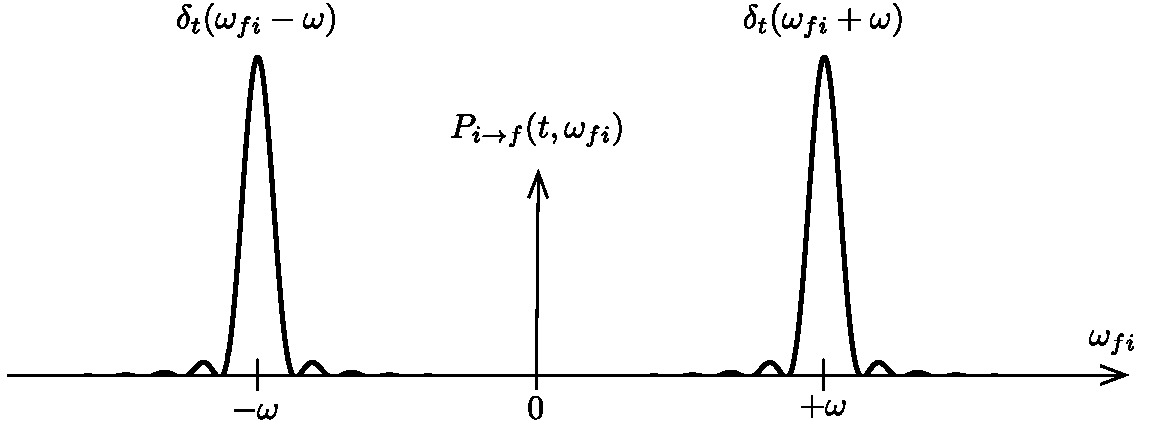
\includegraphics[scale=0.75]{Figs/DoppelSinPlot}
\end{figure}\vspace{-2ex}

Die Goldene Regel für die Übergangsrate im periodischen Fall lässt sich somit schreiben als: 
\begin{eqnarray*}
	\Gamma_{i\rightarrow f} &=& \frac{2\pi}{\hbar} \Big( \big|\bracket{f}{\hat{F}^-}{i}\big|^2\cdot \delta(E_f-E_i-\hbar \omega) + \big|\bracket{f}{\hat{F}^+}{i}\big|^2\cdot \delta(E_f-E_i +\hbar \omega) \Big)
\end{eqnarray*}
Damit gibt es nur Übergänge zwischen Anfangs- und Endzuständen, welche sich um die Energie $\hbar\omega$ unterscheiden. Die Energieerhaltung wird unter Absorption der Endzustandsenergiedifferenz erhalten. Bei Absorption gilt $E_f=E_i+\hbar\omega$ und bei Emission: $E_f=E_i-\hbar\omega$. 

Die Quantenfeldtheorie fordert an dieser Stelle einen Korrekturterm, der im letzten Kapitel behandelt werden wird.

%\end{document}